\documentclass{paper}

\usepackage{xeCJK}

% Formatting
\usepackage{geometry}
\usepackage{titling}
\usepackage{parskip}
\usepackage{float}
\usepackage{tocloft}

% Figures
\usepackage{graphicx}
\usepackage{tikz}
\usepackage{pgfplots}
\usepackage{subcaption}

% Math formulas
\usepackage{amsmath}
\usepackage{esint}

% Hyper refs
\usepackage[hidelinks]{hyperref}

% Bibliography
\usepackage[style=authoryear,backend=bibtex]{biblatex}
\usepackage{filecontents}
% Enlarge the outer brackets of nested formulae.
\delimitershortfall=-1pt

% Bibliography.
\bibstyle{eg-alpha-doi}

% Pseudo code.
\lstdefinestyle{pseudo}{
	mathescape=true,
	extendedchars=true,
	frame=tB,
	breaklines=true,
	tabsize=2,
	numbers=left,
	numberstyle=\tiny,
	basicstyle=\scriptsize,
	keywordstyle=\color{black}\bfseries\em,
	keywords={
		input, output,
		function, datatype,
		return, yield, continue, break
		for, foreach, while,
		do, in, done,
		in, on, from, to,
		if, else,
		begin, end,
		new, delete,
		add, apply,
	},
	numbers=left,
	xleftmargin=.04\textwidth,
}

\title{A Monte-Carlo Method for Realtime Buoyancy Simulation}
\author{}
\date{}

\begin{document}

\maketitle
\begin{abstract}
	Simulating the physical interaction between fluid and solid matter in an interactive application like video games often requires complex algorithms that could be computationally expensive.
	To do it effectively, we proposed a realtime method for calculating the buoyant behavior of solid bodies submerged in fluid based on the Monte-Carlo method.
	Our method can recreate the buoyancy effect realistically while providing the freedom to balance between quality and performance.
	It also takes care of the resistance force as the bodies move through the fluid to prevent numeric instability.
	With proper generalization, this method can be adapted to simulate any fields that solid bodies could move through.

	\begin{keywords}
		solid-fluid coupling; buoyancy; realtime; physical simulation; Monte-Carlo method
	\end{keywords}
\end{abstract}
\section{Introduction}

For a long period of time, \emph{solid-fluid coupling} has been studied as a target of offline algorithms.
For a clip of result to be rendered, it would require a rather long time for the algorithm to process the original data of the physical settings.
Only up to the recent decade, real-time methods start to appear to meet the demand in interactive applications like video games.
As far as we know, it is not easy to simulate this coupling due to the nature of fluid simulation;
it is even harder to accomplish in real-time.

The critical reason that causes the difficulty is that fluid matter doesn't have a fixed shape.
Unlike the nice-and-neat physical interaction between rigid solid objects, the interaction between fluid matter and solid objects could hardly be modeled with a limited number of point-to-point pairs of forces;
instead, fluid matter could morph in space to embrace the submerged objects and cause a net pressuring force on them from many directions.

\begin{figure}[h]
	\begin{center}
		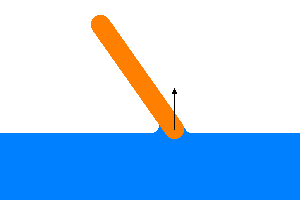
\includegraphics[width=1.3in]{figures/stages-of-a-plank-falling-into-water/1.png}
		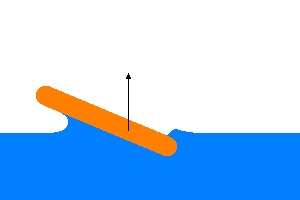
\includegraphics[width=1.3in]{figures/stages-of-a-plank-falling-into-water/2.png}
		
\includegraphics[width=1.3in]{figures/stages-of-a-plank-falling-into-water/3.png}
	\end{center}
	\caption{
		Stages of a plank falling into water.
		Black arrow indicates the net force applied on the plank.
	}
	\label{stages-of-a-plank-falling-into-water}
\end{figure}

Figure \ref{stages-of-a-plank-falling-into-water} shows a simple example demonstrating the complexity:
Assume that a piece of wood plank is falling into water at an angle.
When a side of it first touches the water, that side would immediately get pushed up, resulting in a torque causing the plank to pitch;
then the whole face of the plank will splat itself onto the water surface;
in the last, the plank's momentum is sufficiently decreased and it will slowly sink into or hold still on the water.
To simulate this whole process in a computer, there are two difficulties to be dealt with:

\begin{enumerate}
	\item It is not easy to find the exact volume of the submerged part of a solid object.

		To get the accurate buoyancy force, one would have to find which parts exactly are sunk in the water and keep making queries to the geometrical shape of the solid object.
		Unfortunately, common game engines only provide very limited interfaces on geometry information of physical bodies.
		As a workaround, one could manually iterate through all the surfaces of the physical body's collision mesh, calculate each forces applied on the surfaces, and sum them up.
		This would be a linear performance cost relating to the amount of triangle surfaces of the floating object.
		The more complex the object's geometry is, the longer the algorithm needs to run.

	\item It could be overly expensive or sometimes even impossible to compute.

		Finding only the accurate geometry information isn't enough, as every surfaces could be partially sunk in the water.
		If the algorithm only uses the full area of the surfaces to calculate the buoyancy force, then soon as an object touches the water, it would receive the maximum buoyancy force, which leads to artifacts.
		To avoid this, all surfaces of the mesh must clipped in each time the algoritm runs.
		Not only this would cause more performance cost, it also requires a clear, definite boundary of the water surface to be queried during runtime.
		As the implementation of the water body varies, this might even be impossible to achieve.
\end{enumerate}

In general, to calculate the exact physical effect caused by the surrounding fluid environment, one would have to gather all the information around the whole surface of the target object.
This would often lead to performance issues.
However, although it is difficult to solve the problem directly, in this article we proposed a flexible solution based on the Monte-Carlo method's idea.
It solves the problem by using random sampling, and could get a statistically correct solution under a configurable amount of error due to the randomness introduced by the method.
Because of this method of calculating environmental physical effect is not limited to the case of fluid, it could be easily adapted to other kinds of physical fields.
\section{Related Works}

The study on the physical interaction between solid objects and its surrounding environment could be traced back to an very early stage of Computer Graphics.
Due to the natural complexity of the target, researches has never set their goals on creating a factual realistic result, but only a visual realism.
In the most common practices, solid objects were often modelled as rigid bodies as in \cite{BAR01}; when computing the physical effects, the whole body could be simplified into a single point at its center of mass.
This simplification would cause problems when it comes to buoyancy simulation, as the real geometry of the solid object must be taken into account.
To reach a more realistic result, two styles of approaches have been studied primarily \cite{GOU09}.

\subsection{The Lagrangian Approach}

The Lagrangian approach models the fluid environment into small particles and calculates each of their force contributions on the target solid objects.

A study in 2004 \cite{CAR04} gives an example of Lagrangian approach on fluid-solid coupling simulation.
This approach requires a Lagrangian fluid solver to be present in order to simulate the motion of the fluid itself.
Because solid objects are considered as fluid particles during the solver's working phase, this approach could be suffering from performance issues when the submerged solid objects' geometries frequently change or contain huge amounts of triangles.
Also, it would require the solver to run at a high resolution when the simulation environment is complex, or the simulation might be inaccurate and thus unrealistic.

Another study in 2012 \cite{AKI12} takes a step even further to model not only the fluid matter into small particles, but also the submerged solid bodies' surfaces.
This study could achieve very realistic results, but nowhere meets the demand of interactive simulation.

Due to the heavy computation it requires, the Lagrangian approach is seldomly used in interactive scenarios.

\subsection{The Eulerian Approach}

The Eulerian approach focuses on the physical field created by the existence and motion of the fluid matter.
Their effects on submerged bodies could be thought of the net value on the bodies' surfaces under integration.
Because the Eulerian approach treats the fluid matter as a whole, the heavy computation could be parallelized and performed by GPU, thus it has a great advantage in performance than the Lagrangian approach.

In 2013, an optimized model of a panel-based Eulerian fluid-solid coupling is proposed \cite{GER13}.
The model takes the entire fluid volume as the induced field of a limited amount of ``panels'' -- essentially generating seeds at certain location that represent the surrounding fluid motion in their adjacent spaces.
This model is cheap enough to run at a realtime scale in a 2D game, but sacrifices the accuracy be reducing the freedom of the fluid's behavior.

A study in 2020 \cite{BAJ20} matches our topic the best:
They have proposed a model to simulate the sinking phases of buoyant objects.
Similar to \cite{GER13}, their method uses a seed-based simplification to reduce the heavy computational cost; but the simplification is applied on the solid objects instead of the fluid body.
Their method could result in good visual realism over targets of different sizes, but requires the solid objects to be pre-configured with a seed graph.
If the solid object's geometry changes at runtime, the graph would then be reflecting an incorrect physical proxy, leading to artifacts.

Continuing on previous ideas, our model adapts an Eulerian approach that saves performance by reducing the computation on the net force.
This reduction is achieved by estimating over random samples over the surface of the submerged solid bodies' geometries.
\section{Problems With Archimedes Principle}

Back to 246 BC, the ancient Greek philosopher Archimedes has proposed his famous principle on buoyancy:
\begin{quote}
	Any object immersed in a fluid is subject to an upward buoyancy force equal to the weight of the fluid displaced by the object.
\end{quote}
This princple is correct in most of the cases;
however, there are still some edge cases where it will fail \cite{bierman2003reconsidering} \cite{mohazzab2017archimedes}.
Before showing the cases, we need to understand why the principle holds in the first place.

The net buoyancy force can be seen as the unity of all the pressuring force from surrounding water applied on the floating object.
The strength of water pressure is related to many variables, including the water's density, its velocity field, the local gravity strength, etc.;
but in static water, the pressure (force per unit surface area) at the same height can be seen as the same, proportional to the depth to the water surface, as shown in formula (\ref{static-water-pressure}).
\begin{equation}
	P=\rho gh.
	\label{static-water-pressure}
\end{equation}
where $P$ is the pressure, $\rho$ is the fluid density, $g$ is the local gravity strength, and $h$ is the depth to the water surface.
For each small area $\mathrm{d}s$ with the normal direction $\mathbf n$, the surrounding fluid would cause a pressuring force of $-\mathbf nP\mathrm{d}s$ on it.
We can integrate this around the whole surface to get the net force, given as formula (\ref{net-water-pressuring-force}).
\begin{equation}
	\mathbf{F}_P=\oiint_{S}-\mathbf nP\mathrm{d}s.
	\label{net-water-pressuring-force}
\end{equation}
If the object is fully sunk, we then have that the integrating surface would be the boundary of the object's volume ($S=\partial V$), which is guaranteed to be a 3D manifold.
Under this assumption, using the \emph{divergence theorem} in multi-variable integration, formula (\ref{net-water-pressuring-force}) can be continued as (\ref{archimedes-principle-formula}) \cite{pfeffer1986divergence}.
\begin{equation}
	\mathbf{F}_P=\iiint_{V}\rho\mathrm{d}v=-\rho\mathbf{g}|V|.
	\label{archimedes-principle-formula}
\end{equation}
This yields exactly the Archimedes principle.

Surprisingly, when the object is only partially sunk, this equation still holds;
just that the $V$ now means only the sunk part of the geometry.
The reason that it still holds is because after taking a cut of the geometry at the water surface, the water pressure on the newly cut surface would be zero, since it is overlapping with the water surface.

Together, the two cases make up the Archimedes principle.
They are covering the most cases that most people will ever face, so the principle could be used with no problem.
However, in Figure \ref{archimedes-principle-failing-case} below, Archimedes principle fails to hold on the two orange boxes.

\begin{figure}[h]
	\begin{center}
		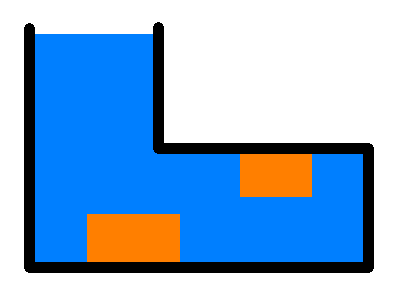
\includegraphics[width=1.3in]{figures/ap-blind-spot.png}
	\end{center}
	\caption{When Archimedes principle fails to hold.}
	\label{archimedes-principle-failing-case}
\end{figure}

Both of the two boxes have one of their surfaces sticking to the wall, but neither of the surfaces are overlapping the water's surface.
This means that if they are really touching the water, they should receive a non-zero pressure.
In these cases, formula (\ref{archimedes-principle-formula}) -- derived from the divergence theorem -- would be incorrectly taking the wall-surfaces' fake pressure into the sum of the net force, thus leading to a wrong result.

To deal with such cases, we could explicitly calculate the original integral following formula (\ref{net-water-pressuring-force}) to get the correct result; but an immediate problem is that it would require us to actually integrate all the infinitesimals.
This is imposible for computers to achieve, so we need to transform them into finite surface fragments \cite{klosek1997integration}.

Most common 3D model formats are based on polygons, so this can be done with no difficulties.
The updated formula is given as (\ref{discretized-pressuring-force}).
\begin{equation}
	\mathbf{F}_P=\sum_{\text{face}}-\mathbf{n}\rho h|\text{face}|.
	\label{discretized-pressuring-force}
\end{equation}

Although this formula can be directly calculated by a computer, it leads to two new problems:
\begin{enumerate}
	\item It could be a huge performance cost to iterate through all surfaces of a mesh.
	\item After discretizing into non-infinitesimal surfaces, the simple-and-nice $\rho h$ for calculating the pressure doesn't hold anymore.
\end{enumerate}

The first problem is rather easy to see;
and the reason for the second problem is that, as though the position for an infinitesimal of the surface is clearly defined, a small surface fragment has its extent in the space.
Most commonly, a surface is not aligned directly to the Y-axis, and the different parts of it would be at different depth, resulting in experiencing different pressure (Figure \ref{water-pressure-differs-on-surface}).

\begin{figure}[h]
	\begin{center}
		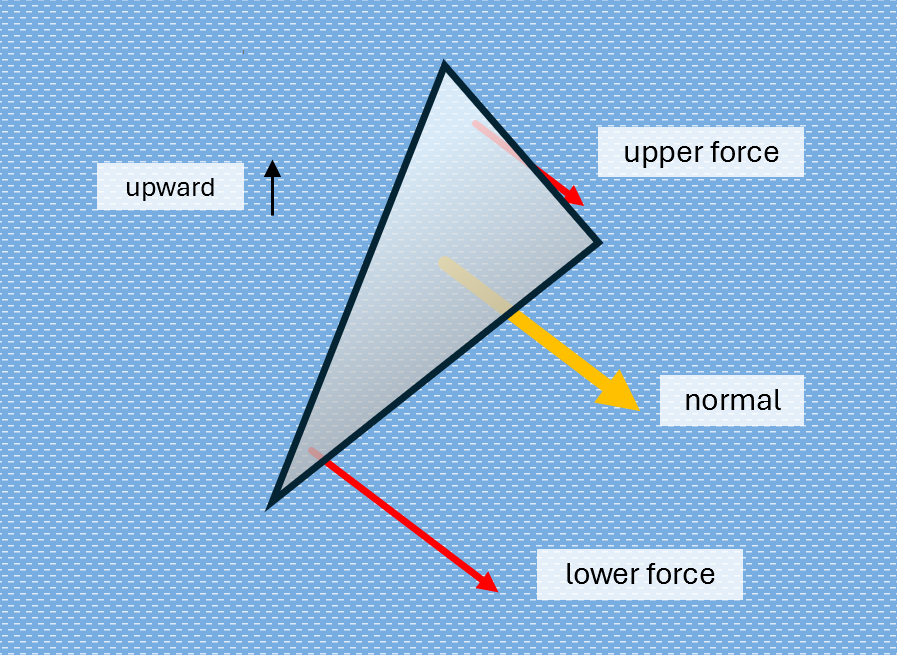
\includegraphics[width=3in]{figures/water-pressure-on-small-surface.png}
	\end{center}
	\caption{The water pressure differs on a surface.}
	\label{water-pressure-differs-on-surface}
\end{figure}
\section{Applying the Monte-Carlo Method}

By using the \emph{Monte-Carlo method}, the above two problems could be resolved.
It is a methodology of using a set of local information on random samples to estimate the accurate value, at a cost of certain amount of noise.
In the case of buoyancy, the force only affects the float object's acceleration directly, which is the second-order derivative of its location;
as the time passes, the noises generated from the randomness could accumulate and statically cancel themselves out.
Therefore, we can use a small set of water pressuring force calculated over random points on the floating body's surface to estimate the net buoyancy force without introducing too much error.

To apply the Monte-Carlo method, there are the following steps:
\begin{enumerate}
	\item Generate random sample points over the surface of the target physical body;
	\item Calculate each of their pressuring forces;
	\item Sum up the forces;
	\item Regularize the summed-up result.
\end{enumerate}

\subsection{Sampling Over the Surface}

As already introduced previously, most game engines have poor interfaces for querying the geometry information of models, so they cannot be relied on. Sampling in the UV space might work, but there are some problems:
\begin{itemize}
	\item
		The area that a triangular face occupies in the UV space doesn't reflect its real area in the world space (or at least in its local space).
		If we were to sample in the UV space, we would have to calculate a conversion ratio to convert the area between the two spaces, like the Jacobian determinant when changing an intergral variable.
	\item Even if we do calculate the conversion ratio, there could be some faces with an zero area in the UV space.
		If this happens, such face could never possibly be sampled and thus is missing from the buoyancy calculation, which will lead to artifactual result.
\end{itemize}

One possible workaround is to generate the samples directly on the triangular faces in the world space.
\begin{itemize}
	\item For each sampling chance, first randomly choose a triangular face to sample on.
		This is completely doable by accessing the basic model information.
	\item Then, uniformly pick a pick a random point on the chosen face.
		Given that the face is a triangle, this step is trivial.
\end{itemize}

After following these steps, there is only one problem remaining:
Every faces would share the same probability to be chosen, yet they are of different sizes.
This is not desired, as a bigger face would receive bigger pressuring force in water;
but under the same probability, they would have the same contribution to the net pressuring force.
To solve this, an approach of weighted average could be applied.
\begin{itemize}
	\item We grant each sample point a weight that equals to the area of the triangluar face it lands on, so that the samples on bigger faces would make bigger contribution of force;
	\item And after all contributions are summed up, the weight sum would be divided from the totaol contribution.
\end{itemize}

An important trait of a Monte-Carlo approach is that the balance between quality and performance can be adjusted.
The higher the sample rate, the better the resulting quality, but it might cause a burden on performance;
vice versa, one could decrease the sample rate and sacrifices the quality to get a better performance.

\subsection{Calculating the Force on Each Sample}

Once we have the whole surface of the body model sampled, we can calculate the local water pressure forces applied on the samples.
Similar to equation (\ref{discretized-pressuring-force}), the pressure force for a sample point would be (\ref{sample-pressure-force}).
\begin{equation}
	\mathbf{f}_{\text{pressure}}(s)=
	\begin{cases}
		-\mathbf{n}\rho h \ \text{if under water}, \\
		\mathbf{0} \ \text{otherwise}.
	\end{cases}
	\label{sample-pressure-force}
\end{equation}
Here the small $\mathbf{f}$ is used to indicate that this is the force on a single face, not the net force.

The weighting coefficient for each sample would be the area of the face that it lands on (formula (\ref{sample-weight})), as discussed in the previous section.
\begin{equation}
	w(s)=|\text{face}|.
	\label{sample-weight}
\end{equation}
Lastly, to sum them all up and get the regularized result:
\begin{equation}
	\mathbf{F}_{\text{pressure}}=\frac
		{
			\bigoplus_{s}
			\left(
				w(s)\cdot\mathbf{f}_{\text{pressure}}(s)
				,
				\text{arm}(s)
			\right)
		}
		{\sum_{s}w(s)}.
	\label{net-pressure-force}
\end{equation}
Where the $\text{arm}(s)$ is the position displacement from the sample point to the center of the body's mass.

Notice that here to add the forces together along with their positions, the $\bigoplus$ symbol is used instead of $\sum$, which is kind of a non-standard usage.
This is because that forces applied on a physical body \emph{at specific locations} can not be simply added together.

\subsection{Composing the Forces Together}

In figure \ref{force-pair}, a pair of opposite forces is applied on the same body, but displaced from its center of mass.
Under the effect of the two forces, the body would rotate in place, but not move at all.
Such pair of opposite forces will not cause any movement on a physical body, but only the rotation.
If only the forces are added together, a zero vector would be expected as the result; all information about the rotation would be lost.

\begin{figure}[h]
	\centering
	\scalebox{0.8}{
		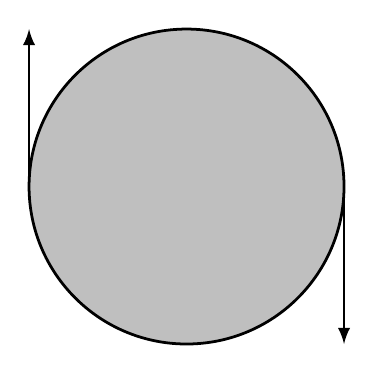
\begin{tikzpicture}
			\filldraw[color=black, fill=lightgray, line width=1pt] (0,0) circle (2);
			\draw[-latex, line width=1pt] (2,0) -- ++(0,-2);
			\draw[-latex, line width=1pt] (-2,0) -- ++(0,+2);
		\end{tikzpicture}
	}
	\caption{An opposite pair of forces applied on a round body.}
	\label{force-pair}
\end{figure}

In general, the net physical effect on a body can be broken down into a force and a torque.
Both of them are equivalently applied on the center of the mass, so that their exact position don't need to be explicitly taken care of.
Given a positioned force $(\mathbf{f}, \mathbf{r})$, where $\mathbf{f}$ is the force and $\mathbf{r}$ is the vector from the center of mass to the point of effect, the equivalent force-torque tuple on the center of mass can be calculated by the following formulae (\ref{positioned-force-to-force-torque-tuple}).

\begin{equation}
	(\mathbf{f},\mathbf{r})_{\text{positioned force}}
	\mapsto
	(\mathbf{f},\mathbf{r}\times\mathbf{f})_{\text{force-torque tuple}}.
	\label{positioned-force-to-force-torque-tuple}
\end{equation}

And to compose two force-torque tuples, simply sum them up component-wise (\ref{composing-two-force-torque-tuples}).

\begin{equation}
	(\mathbf{f}_1,\mathbf{\tau}_1)
	\oplus
	(\mathbf{f}_2,\mathbf{\tau}_2)
	=
	(\mathbf{f}_1+\mathbf{f}_2,\mathbf{\tau}_1+\mathbf{\tau}_2).
	\label{composing-two-force-torque-tuples}
\end{equation}

By applying this into formula (\ref{net-pressure-force}), the net water pressure force could then be calculated.
\section{Introducing the Resistance Forces}

In reality, objects moving through fluid would gradually lose their kinetic energy due to the resistance between its surface and the water body.
If this mechanism is missing, then an object in water might oscillate forever and cannot tend to a still state, which is artifactual.
Also, our method is discretized, meaning that there might be floating-point precision errors introduced within every calculation steps.
If not dealt with, these errors could potentially cause the physical system's energy to continuously accumulate and thus breaking the energy conservation law.
Therefore, we would like this energy-losing mechanism to be added into our model by introducing some resistance components.

The total resistance force of a solid object moving fluid, formally called \emph{parasitic drag}, is a combination of two separate sources of force:
\begin{itemize}
	\item The form drag, or pressure drag, due to the size and shape of the object.
	\item The skin friction drag, or viscous drag, due to the friction between the fluid and the surface of the object.
\end{itemize}

\subsection{Form Drag}

The form drag is caused by the surface of an object being pushed by the fluid blocking on its moving path.
It is proportional to the square of the relative velocity between the moving object and the fluid.
The formula is given as (\ref{form-drag}); the letter $\mathbf{D}$ is used to represent a drag force.

\begin{equation}
	\mathbf{D}_{\text{form}}=\frac{1}{2}\,\rho\,u^2\,c_f\,A,
	\label{form-drag}
\end{equation}
where:
\begin{itemize}
	\item $\rho$ is the mass density of the fluid;
	\item $u$ is the flow velocity relative to the object;
	\item $c_f$ is the drag coefficient, a dimensionless coefficient that depends on the fluid's properties;
	\item $A$ is the area of the object's cross section perpendicular to $u$.
\end{itemize}

This formula is only suitable for calculating a rough net drag force for a whole object;
for our application, we need to adapt it into a form that can be calculated on the sample points.
This could be rather easily done by ``translating'' the terms in (\ref{form-drag}).
\begin{itemize}
	\item $\rho$ remains the same.
	\item $u$ would be the velocity of the body \emph{at the sample point}.
		The position matters because the body might be rotating; in which case the world velocity of each point would differ.
	\item $c_f$ remains the same.
	\item $A$ would be the perpendicular area of the triangular face that the sample lies on.
		This can be calculated by multiplying the real area of the face with the dot product of its normal and the unit vector long $u$.
\end{itemize}

The form drag on each sample point is given as formula (\ref{sample-form-drag}).
\begin{equation}
	\mathbf{d}_{\text{form}}=\frac{1}{2}\,\rho\,\mathbf{v}^2\,c_f\,|\text{area}|\,(\hat{\mathbf{v}}\cdot\mathbf{n}).
	\label{sample-form-drag}
\end{equation}

One important note is that if a face is \emph{not} repelling the fluid in front of it when moving, it should not produce any form drag.
This can be checked by the dot product during the calculation of $A$: if the product is positive, simply drop the drag or make it zero.

\subsection{Viscous Drag}

The viscous drag is caused by the friction between the fluid and the object's surface as the surfaces passes along \emph{parallelly}.
Similar to the form drag, the viscous drag is also proportional to the square of the flow velocity.
The rough formula of a net viscous drag is given as formula (\ref{viscous-drag}).
\begin{equation}
	\mathbf{D}_{\text{viscous}}=\int_{\partial V}\frac{1}{2}\,\rho\,\mathbf{v}^2\,c_v\,\text{d}A.
	\label{viscous-drag}
\end{equation}
It might looks different from (\ref{form-drag}), but really it is the same thing written under the notation of integral.

The formula for the viscous drag on each sample point can be copied from (\ref{sample-form-drag}), but the coefficient needs to be changed, and the dot product should be replaced by the ``parallelliness'' between the face and the flow velocity, which can be given by the absolute value of the cross product.
The formula is given as (\ref{sample-viscous-drag}).
\begin{equation}
	\mathbf{d}_{\text{viscous}}=\frac{1}{2}\,\rho\,\mathbf{v}^2\,c_v\,|\text{area}|\,|\hat{\mathbf{v}}\times\mathbf{n}|.
	\label{sample-viscous-drag}
\end{equation}

\subsection{Integrating Into the Model}

To integrate the resistance forces into our model, we can substitute the sample force term in (\ref{net-pressure-force}) to make it contain the new forces.
The new formula is given as (\ref{net-water-force}).
\begin{equation}\begin{split}
	\mathbf{F}_{\text{all}}=\frac
		{
			\bigoplus_{s}
			\left(
				w(s)\cdot\mathbf{f}_{\text{all}}(s)
				,
				\text{arm}(s)
			\right)
		}
		{\sum_{s}w(s)},
	\\
	\mathbf{f}_{\text{all}}=\mathbf{f}_{\text{pressure}}+\mathbf{d}_{\text{form}}+\mathbf{d}_{\text{viscous}}.
	\label{net-water-force}
\end{split}\end{equation}

Lastly, to ultimately suppress any potential unrealistic energy outbreak, such as a body bouncing back into the sky, one could forcefully apply a energy dissipation of any objects submerged in fluid.
This could be achieved by applying a force and a torque in the opposite direction of the object's velocity and angular velocity continuously in every frame.
The intensity of the force could be controlled by an configurable coefficient.
\section{Implementation and Application}

From the realistic rivers and oceans in the open world games to small water mechanism in puzzle games,
water is a common element of the background settings in many video games.
However, the types of object that could interact with water or the ways that they can do so in games are usually very limited.
Apart from the designs of the game, one big factor limiting the freedom of the interaction with water is on the technical side \cite{kellomaki2012water}.
Due to technical limitations, game developers lack the ways to fully simulate the water interactions and have to often manually overwrite the physical behaviors, which inevitably causes critical glitches \cite{RedditAssassin}.
With our method, game developers could arbitrarily put objects into water bodies without having to worry about physical glitches.

To apply out method into a game project, it is adviced to write a controller class for the water bodies, and let them be the source of the buoyancy forces;
doing so could avoid having to add a ``buoyancy force receiver'' on every single solid objects.
The water body controller does mainly two things:
\begin{enumerate}
	\item Maintain a collection of all solid objects that are submerged in this water body.
	\item Calculate and apply the forces contributed by the water body onto the objects in each physical frame.
\end{enumerate}

In each physical frame, the brief outline of the water body controller's tasks is given as Table \ref{water-controller-main-loop}.

\begin{table}[htb]
	\centering
	\begin{lstlisting}[style=pseudo]
		input sampleDensity
		input submergedBodies
		do in every physical frame
			foreach body in submergedBodies
				surfaceArea := CalculateSurfaceArea(body)
				sampleCount := surfaceArea * sampleDensity
				samples := SampleOverSurface(body, sampleCount)
				effects := new List
				add MakeBuoyancies(body, samples) to effects
				add MakeResistances(body, samples) to effects
				netEffect := $\bigoplus$ effects
				apply netEffect on body
			done
		done
	\end{lstlisting}
	\caption{The main loop of the water controller.}
	\label{water-controller-main-loop}
\end{table}

And the data type of the samples output by \texttt{SampleOverSurface} is defined as in Table \ref{surface-sample-data-def}.
Both the position and the normal vectors should in the world space instead of the physical bodie's local space, because that is where the calculations take place.

\begin{table}[htb]
	\centering
	\begin{lstlisting}[style=pseudo]
		datatype SurfaceSample
			position: Vector
			normal: Vector
			area: float
			weight: float
		end
	\end{lstlisting}
	\caption{The type definition for a sample on the surface.}
	\label{surface-sample-data-def}
\end{table}

It is important to feed the samples al at once in to the functions that compute the physical effects such as \texttt{MakeBuoyancies} and \texttt{MakeResistances}, since they need to accumulate the weights of the samples to normalize them before returning.

Table \ref{mesh-sampling-algorithm} gives an algorithm for generating random samples over a mesh.

\begin{table}[htb]
	\centering
	\begin{lstlisting}[style=pseudo]
		function SampleOverSurface
			input body
			input count
			vp := body.mesh.vertexPositions
			foreach i from 0 to count-1
				ti := random integer from 0 to body.mesh.triangleCount-1
				triangle := [vp[ti+0], vp[ti+1], vp[ti+2]]
				foreach position in triangle
					position = body.localToWorldMatrix * position
				done
				i = triangle[1] - triangle[0]
				j = triangle[2] - triangle[0]
				cross = i $\times$ j
				area = 0.5 $\times$ cross.magnitude
				yield new SurfaceSample {
					position = SampleInTriangle(triangle)
					normal = Normalize(cross)
					area = area
					weight = area
				}
			done
		end
	\end{lstlisting}
	\caption{The algorithm for generating random samples over a mesh.}
	\label{mesh-sampling-algorithm}
\end{table}

Figure \ref{boat-sample} shows an example of an application of a boat floating on the sea.
Without having to write any additional codes, just by keeping loading heavy balls onto the boat, the sunk depth of the boat automatically increases.

\begin{figure}[htb]
	\centering
	\begin{subcaptionblock}{0.46\textwidth}
		\centering
		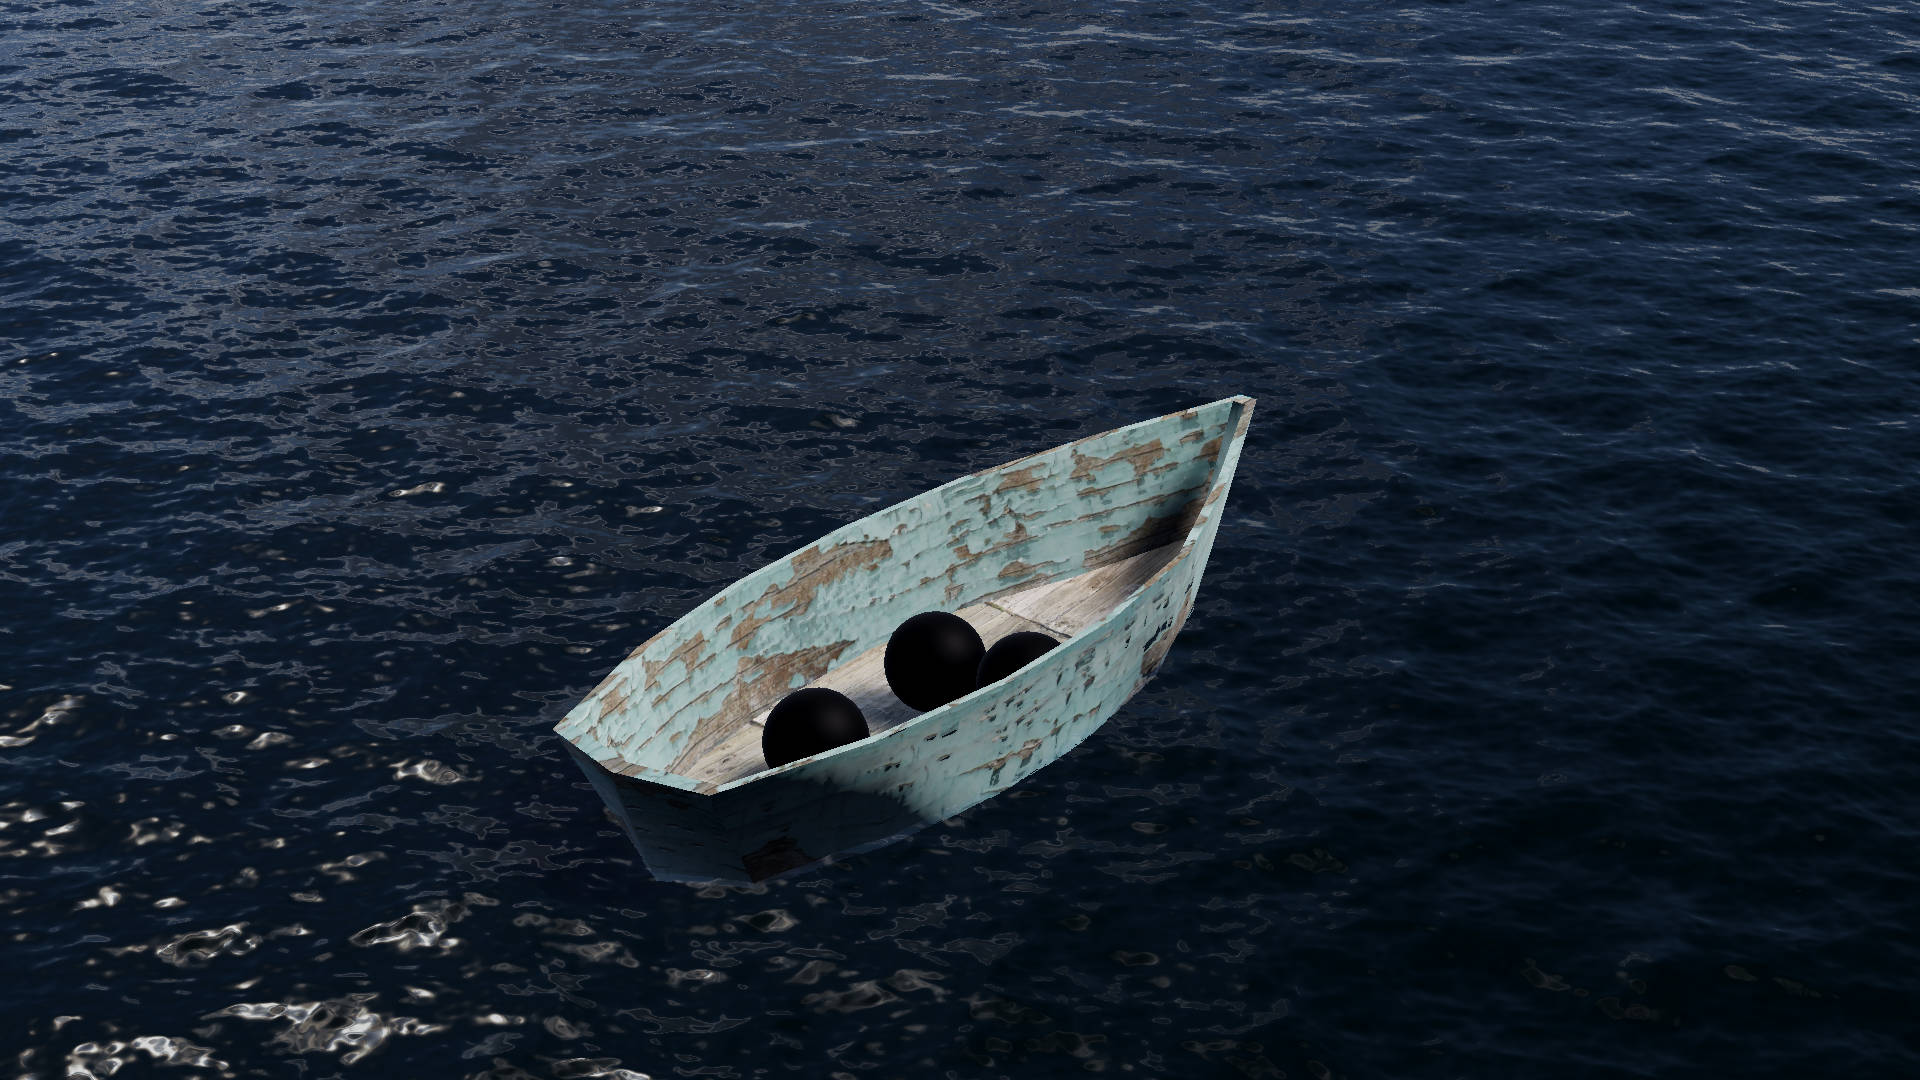
\includegraphics[height=1in]{figures/light-boat.jpg}
		\caption{A boat containing a few balls.}
	\end{subcaptionblock}
	\begin{subcaptionblock}{0.46\textwidth}
		\centering
		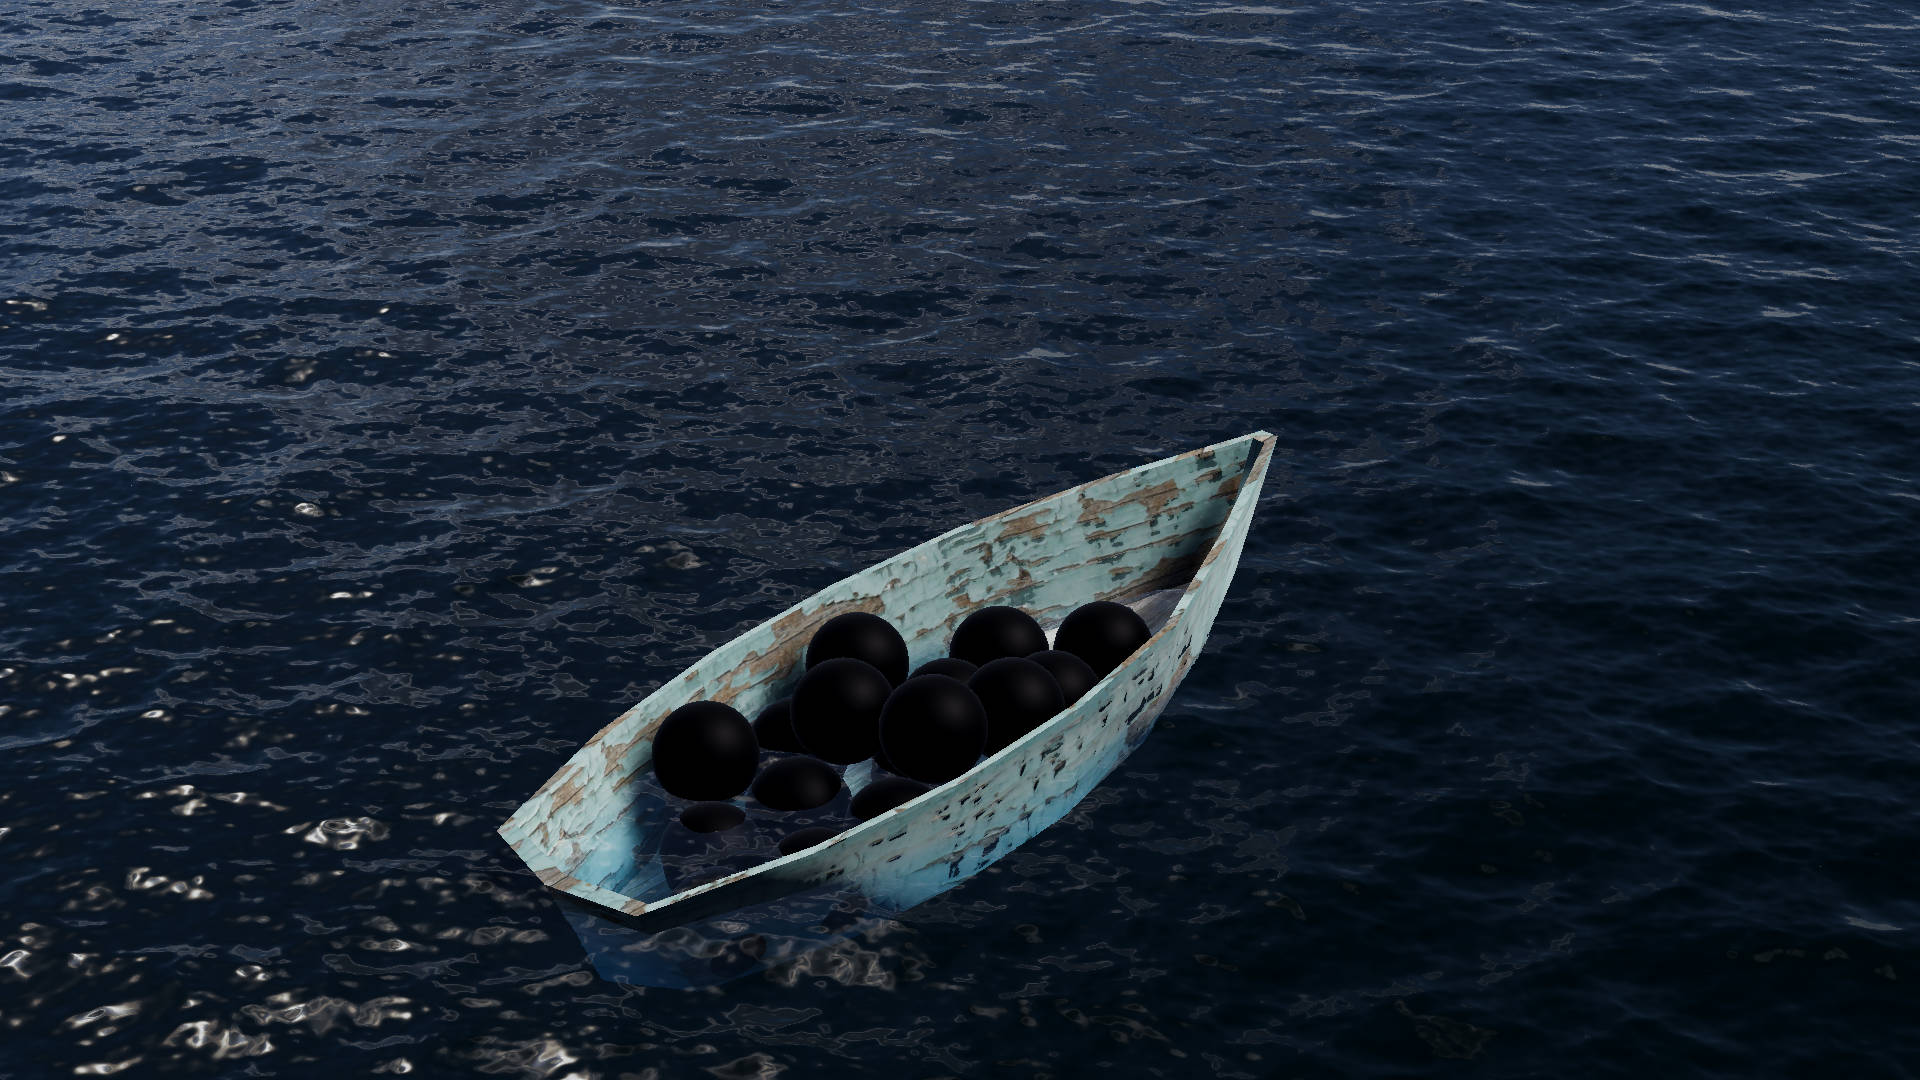
\includegraphics[height=1in]{figures/heavy-boat.jpg}
		\caption{The same boat containing many balls.}
	\end{subcaptionblock}
	\caption{Loading more balls onto the boat increases its depth.}
	\label{boat-sample}
\end{figure}

When applied in real game design, this extra freedom could allow game designers to create more complex mechanisms.
It is clear that often an open mechanism tends to lead to emergent behaviors \cite{sweetser2006emergent}, thus increasing the fun of the game.

Buoyancy simulation could also be used for creating the vibes.
Figure \ref{floating-donut-in-game} shows a screenshot of a poolcore-themed puzzle game, in which water is a main part of the visual design.
Adding objects that could float on water definitely helps emphasize the vibes of the pools.

\begin{figure}[ht]
	\centering
	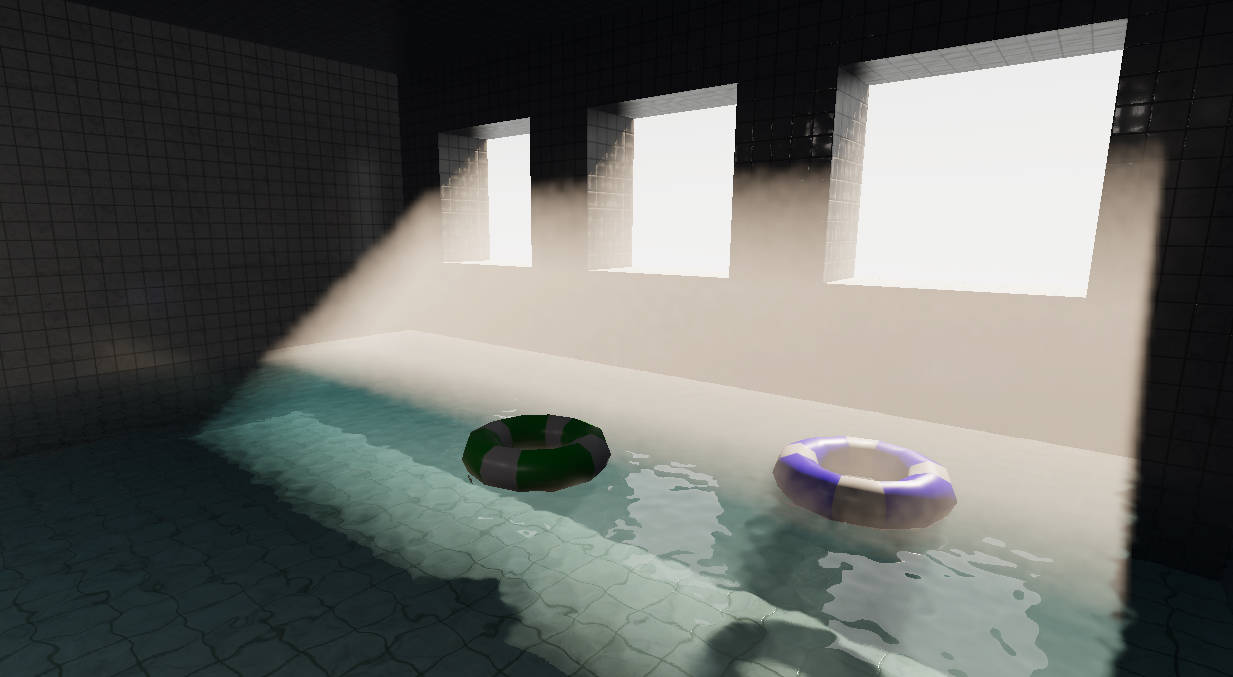
\includegraphics[width=0.4\textwidth]{figures/floating-donut-in-game.jpg}
	\caption{Floating objects can be seen in a poolcore-themed game.}
	\label{floating-donut-in-game}
\end{figure}
\section{Experiment and Analysis}

All below experiments are setup with the Unity engine (version 2022.3.29f1) running on a PC on Windows 11.
The device runs on a CPU of 13th Gen Intel(R) Core(TM) i9-13900HX at 2.20 GHz with 16.0 GB of RAM.

\subsection{Experiment (a): Realism}

To test if the model could realistically simulate the buoyancy force, an experimental simulation immitating the scenario introduced at the beginning of the article where a plank falls into the water is setup.
There are two aspects with which we can judge whether the model is succesful or not:
\begin{enumerate}
	\item Will the plank float back to the water surface and oscillate up and down until it reaches a stable state?
	\item Will the plank turn its flat face up under the influence of the buoyancy force?
	\item If the resistance terms are omitted, will the plank oscillate forever whilst the kinetic energy is conserved?
\end{enumerate}

\paragraph{Environment Setup}

In a Unity scene, a block of static water is placed amid the empty space.
A piece of plank is put above the water surface for a couple of meter's height (figure \ref{simulation-environment}).
The plank's density is made to be lighter than the water density so that it floats.
The water block is wide and deep enough so that the plank would never touch the other faces except the top face.

\begin{figure}[h]
	\centering
	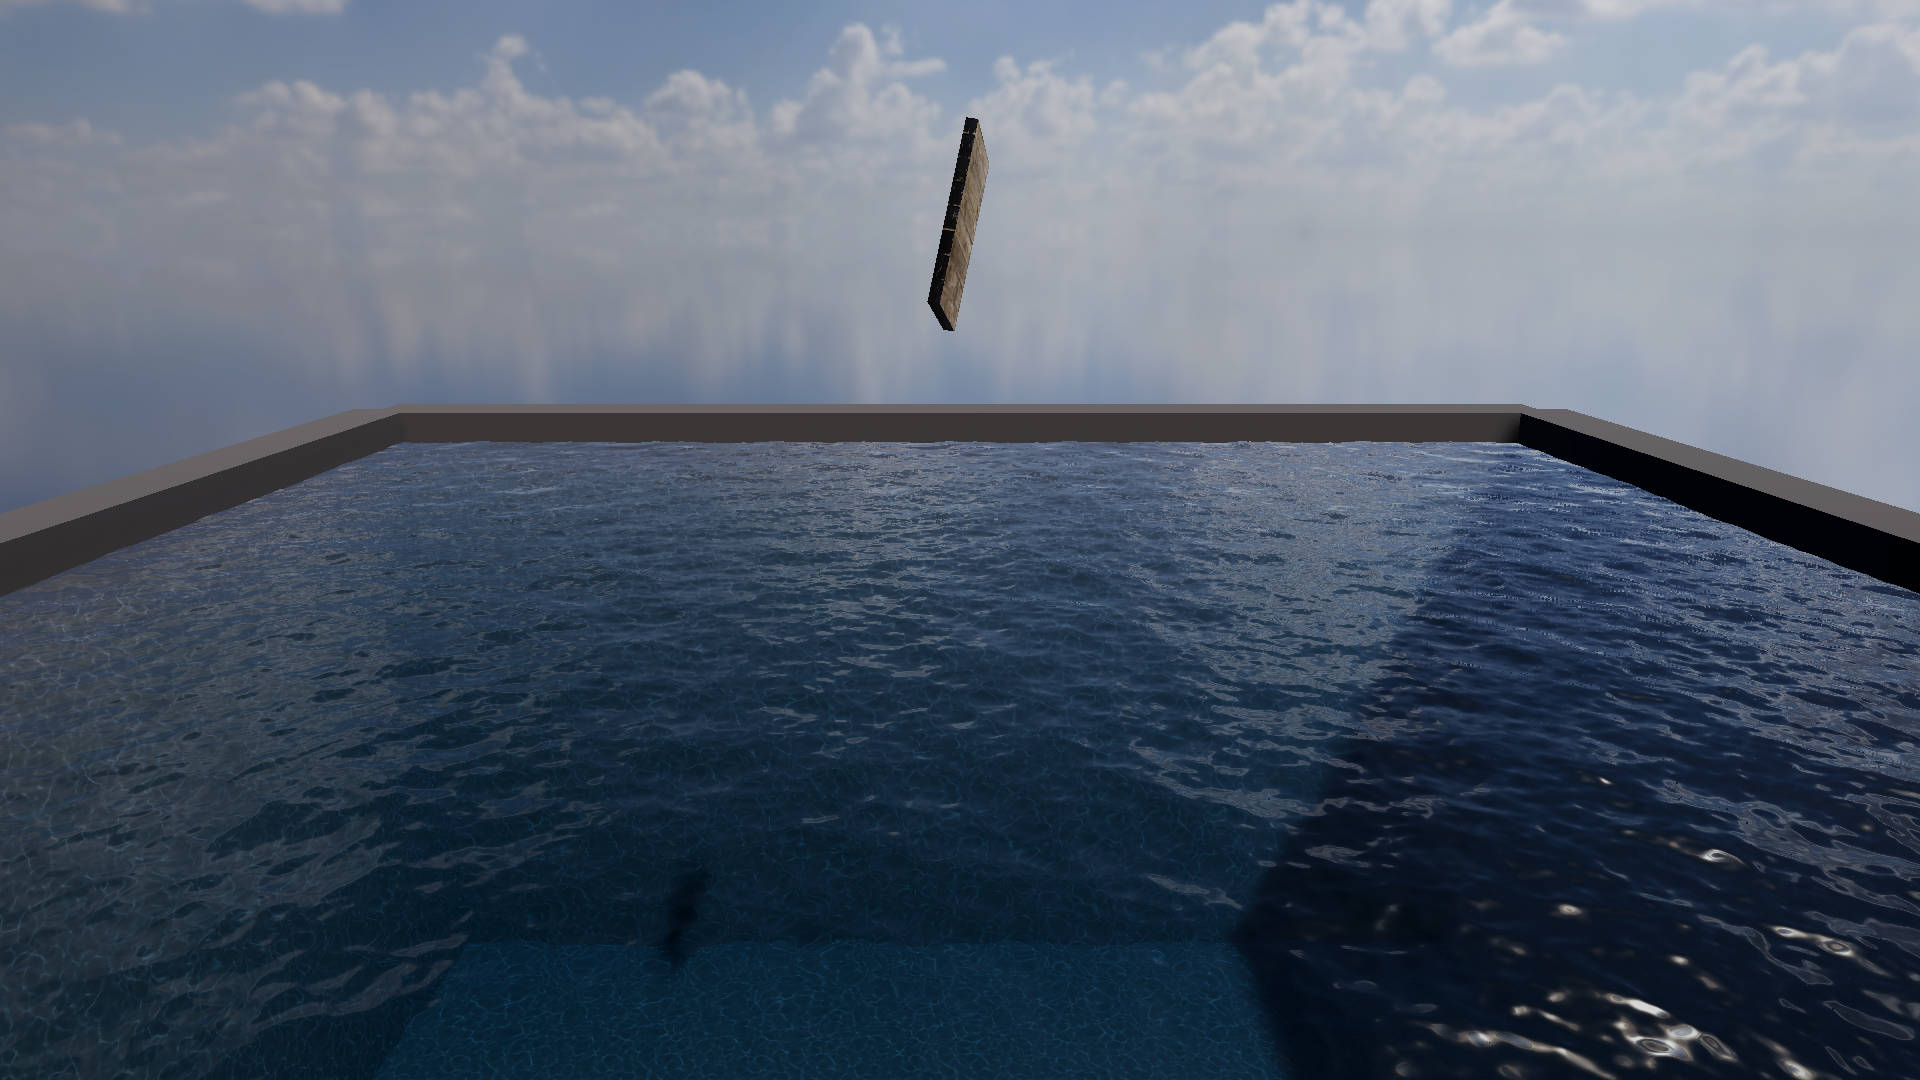
\includegraphics[height=2.5in]{figures/experiment-environment.jpg}
	\caption{The simulation environment.}
	\label{simulation-environment}
\end{figure}

The properties of the water is given in table \ref{simulation-water-properties}.

\begin{table}[h]
	\centering
	\begin{tabular}{ c c c c }
		\hline
		$\rho$ {\footnotesize(density)} & $c_f$ {\footnotesize(form drag coef.)} & $c_v$ {\footnotesize(visc. drag coef.)} & {\small dissipation coef.} \\
		\hline
		1.33 & 0.1 & 0.1 & 1.0 \\
		\hline
	\end{tabular}
	\caption{The properties of the water used in the simulation.}
	\label{simulation-water-properties}
\end{table}

The sampling rate is set at 200 samples per physical frame.

\paragraph{The Process}

At the beginning of the simulation, the plank is let go free-falling into the water.

During the whole process of the simulation, the critical physical properties of the plank will be recorded in every frame for later analysis.

The simulation will stop at an appropriate time after a relatively stable state is reached.

\paragraph{Result}

Figure \ref{simulation-result-heights} shows the position of the plank relative to the water surface during the fall.
The olive-colored line shows the position of the plank's center-of-mass, while the blue line shows the height of the lowest point on the plank.
Figure \ref{simulation-result-rot} shows the pitch angle of the plank during the fall.

\begin{figure}[htb]
	\centering
	\begin{subcaptionblock}{0.48\textwidth}
		\centering
		\fbox{
			\scalebox{0.65}{
				\begin{tikzpicture}
					\begin{axis}[
						width=5in, height=3in,
						enlargelimits=false,
						xlabel={time (seconds)},
						ymin=-2, ymax=5, ytick={-2,-1,...,5},
					]
						\addplot[black] coordinates { (0,0) (5,0) };
						\addplot[olive] table[x=t, y=com] {figures/simulation-record.dat};
						\addplot[blue] table[x=t, y=min] {figures/simulation-record.dat};
					\end{axis}
					\matrix [draw, below left, fill=white] at (4.25in, 2.25in) {
						\node[olive, font=\footnotesize] {center-of-mass}; \\
						\node[blue, font=\footnotesize] {lowest point}; \\
					};
				\end{tikzpicture}
			}
		}
		\caption{The position of the plank during the fall.}
		\label{simulation-result-heights}
	\end{subcaptionblock}
	\begin{subcaptionblock}{0.48\textwidth}
		\centering
		\fbox{
			\scalebox{0.65}{
				\begin{tikzpicture}
					\begin{axis}[
						width=5in, height=3in,
						enlargelimits=false,
						xlabel={time (seconds)},
						ylabel={pitch (degree)},
						ymin=0, ymax=90, ytick={0,15,...,90},
					]
						\addplot[color=red] table[x=t, y=rx] {figures/simulation-record.dat};
					\end{axis}
				\end{tikzpicture}
			}
		}
		\caption{The rotation of the plank during the fall.}
		\label{simulation-result-rot}
	\end{subcaptionblock}
	\caption{The simulation data captured from experiment (a).}.
	\label{simulation-result}
\end{figure}

From the figures we can see, soon as the plank touches the water surface (the blue line intersects with the black horizontal line), it immediately started to rotate (the red line rises) so that its flat face is splatted onto the water surface;
meanwhile it started perceiving an upward buoyancy force, repulsing it from continuing falling (the olive line starts accelerating upwards).
Eventually, the plank floats up to the water surface and oscillates to a stable state (the olive line tends to be horizontal);
also, the plank's flat face is aligned to the water surface (red line approaches $y=90$).

Figure \ref{experiment-no-resistance} shows a clip of the simulation result when the resistance terms are omitted by setting the drag and  dissipation coefficients to zero.
It can be seen from the olive line that the plank will indeed oscilate forever whilst keeping its kinematic energy.

\begin{figure}[htb]
	\centering
	\fbox{
		\scalebox{1}{
			\begin{tikzpicture}
				\begin{axis}[
					width=6in, height=2in,
					enlargelimits=false,
					xlabel={time (seconds)},
					ymin=-5, ymax=5, ytick={-5,-4,...,5},
				]
					\addplot[black] coordinates { (0,0) (10,0) };
					\addplot[olive] table[x=t, y=com] {figures/no-resistance.dat};
					\addplot[blue] table[x=t, y=min] {figures/no-resistance.dat};
				\end{axis}
				\matrix [draw, below left, fill=white] at (5.25in, 1.25in) {
					\node[olive, font=\footnotesize] {center-of-mass}; \\
					\node[blue, font=\footnotesize] {lowest point}; \\
				};
			\end{tikzpicture}
		}
	}
	\caption{The resistance-free simulation data captured from experiment (a).}.
	\label{experiment-no-resistance}
\end{figure}

Based on the analysis of the result, we can say that our model has met the desired experiment result and is indeed succesful.

\subsection{Experiment (b): Performance}

The performance of our method could be tested by keep spawning new buoyant objects and tracking the FPS.

\paragraph{Environment Setup}

The water body remains the same as in the above experiment, except that the sample rate is decrease to 20 samples per physical frame.
An automatic object spawner is placed above the water surface, which will spawn new planks constantly at a custom rate (figure \ref{spawner-setup}).

\begin{figure}[h]
	\centering
	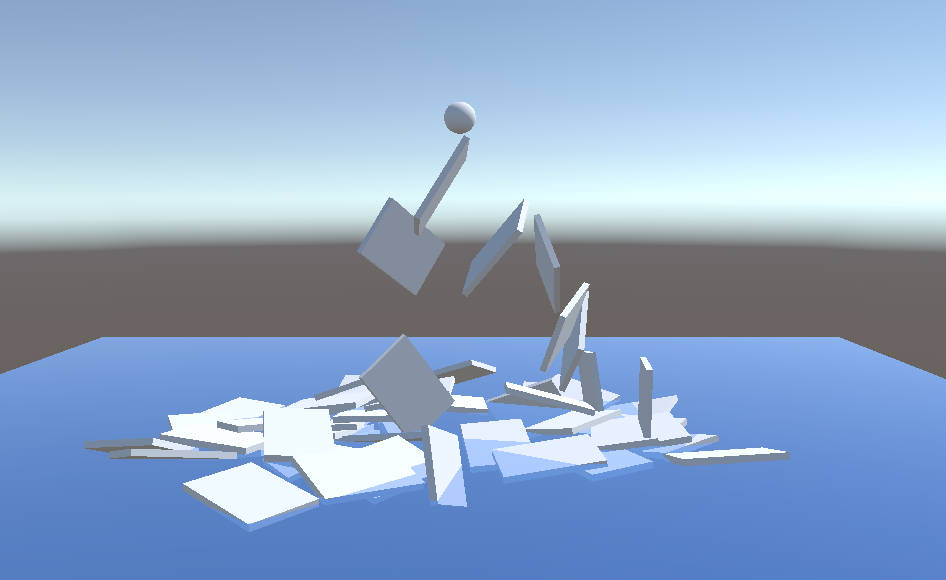
\includegraphics[height=2in]{figures/spawner-setup.jpg}
	\caption{A screenshot of the working object spawner.}
	\label{spawner-setup}
\end{figure}

\paragraph{The Process}

Soon as the game starts, the object spawner would start working and dropping planks into the water.
The number of spawned planks, the time since start and the FPS corresponding to the time would be recorded in realtime.
Also, we would provide another set of FPS record of the same environment but without the presence of the water body as the comparison in order to clearly see the performance cost caused by our method instead of other environmental factors.

\paragraph{Result}

Figure \ref{experiment-spawner} shows the change of FPS as more and more planks are spawned and dropped into the water body.

\begin{figure}[htb]
	\centering
	\fbox{
		\scalebox{0.75}{
			\begin{tikzpicture}
				\begin{axis}[
					width=6in, height=3in,
					enlargelimits=false,
					xlabel={time (seconds)},
					xmin=0, xmax=5,
					ymin=0, ymax=500,
					axis y line*=left,
					ylabel=FPS
				]
					\addplot[blue] table[x=t, y=fps] {figures/spawner-real.dat};
					\addplot[gray] table[x=t, y=fps] {figures/spawner-compare.dat};
				\end{axis}
				\begin{axis}[
					width=6in, height=3in,
					enlargelimits=false,
					xmin=0, xmax=5,
					ymin=0, ymax=50,
					ylabel=number of objects
					axis y line*=right,
					ylabel near ticks, yticklabel pos=right,
				]
					\addplot[red] table[x=t, y=n] {figures/spawner-real.dat};
				\end{axis}
				\matrix [draw, below right, fill=white] at (0.25in, 2.25in) {
					\node[blue, font=\footnotesize] {control}; \\
					\node[gray, font=\footnotesize] {comparison}; \\
				};
			\end{tikzpicture}
		}
	}
	\caption{The performance data collected from experiment (b).}.
	\label{experiment-spawner}
\end{figure}

From the result we can see that our method would cause a linear cost on the performance as the number of submerged objects increases.
At around the time when the amount of objects exceeds 30, it would drag the performance down for about 50\% under the current environment.

In conclusion, our method is suitable for simulations where there are a moderate amount of submerged objects;
it may cause a performance burden if there are too much objects at the same time.

% \subsection{Experiment (c): Complex Geometry}

% The goal of this experiment is to test if our method is working well on target objects with complex geometries, as this is often a disadvantage of other Eulerian approaches that are based on simplified geometries.
\section{Conlusion and Discussion}

Starting from digging into Archimede's law, we managed to build a realistic model of the buoyancy force on solid bodies submerged in fluid.
To overcome the difficulties on discretization, we then apply the Monte-Carlo method on the model.
By doing so, the model yields into a practical algorithm that can freely balance between quiality and performance.
To make it more realistic, we introduced the resistance terms into the model.
After generalizing, the model can even support from introducing custom physical contributions to simulating other kinds of field interaction.
In the last, we put the model on a run and verified its feasibility.
The result shows that the model is capable for simulating the buoyancy force on submerged bodies in an interactive application at real-time.

\paragraph*{Generalization}

Although our model is proposed mainly based on the assumption of a static water body,
the key formula (\ref{net-water-force}) is, however, completely irrelevant to this assumption.
It is fundamentally a Monte-Carlo method to simulate the effect of any fleid on a rigidbody.
One should be able to easily substitute the $\mathbf{f}_{\text{pressure}}$ term with their own version to make it compatible with a more complex implementation of the water body, for example, a particle or height field based water system; or substitute the entire $\mathbf{f}_{\text{all}}$ term to simulate other kinds of fields like a wind blow or magnetic field.

\paragraph*{Limitations}

Our model only provides a solution to one half of fluid-solid coupling -- how solid objects move in fluid.
It is unable to use our model to simulate the backward effect that the solid object causes to the fluid.

Our model runs on CPU and would thus suffer performance cost when there are many objects to simulate.
One could try to optimize the performance in the following directions:
\begin{itemize}
	\item Finding a way to parallelize the computation.
	\item Optimize the computation for fully-submerged bodies.
\end{itemize}

When running under a low sample rate, the model could result in instability.
The random nature of the model would unevitably introduce noise into the physical outcome, leading to a Brownian-like vibrating behavior.
This could appear artifactual, especially when the submerged body is close to the stable state.

To avoid artifacts, one way is to increase the sample rate, but it would increase the cost on performance;
another way is to use stabilizing or filtering algorithms.
Doing so might introduce delay in the physical response;
but depends on the actual application, the downstream developers shall be able to choose the best choice on their own.

\begin{comment}
\section*{Postscripts and Acknowledgements}

This is the first time I have ever written a serious academical article.
It is guaranteed that there will be naive mistakes all over the place.
Please excuse me, thou reader.
If thou hast spotted any mistake, please feel free to contact me at \url{wangnianyi2001@outlook.com}.
My apologies in advance!

Thanks to the team of my graduation project, \emph{Nani Core} (\url{https://github.com/nani-core}).
The idea of this article rose when I was making the water system in the project.
They established the possibilty for this article to happen.
Special thanks to 陈恩晖 (Omnisch) and 张嘉玥 (Limko).
They are two really, really reliable co-workers and good friends of mine.
They have given me the greatest mental and physical support on the project, and an unforgetful memory in my graduation year.
\end{comment}

\begin{comment}
	\section*{Appendix}

	A sample project of the simulation experiment is published at \url{https://github.com/WangNianyi2001/Water-Simulation-2024}.
\end{comment}
\filecontents{references.bib}
@article{BAR01,
  title={Rigid body simulation},
  author={Baraff, David},
  journal={SIGGRAPH Course Notes 1992},
  volume={19},
  year={2001},
  publisher={Citeseer}
}

@article{GOU09,
  title={Fluid simulation for video games (part 3)},
  author={Gourlay, Michael J},
  journal={Intel online articles},
  year={2009}
}

@article{CAR04,
  title={Rigid fluid: animating the interplay between rigid bodies and fluid},
  author={Carlson, Mark and Mucha, Peter J and Turk, Greg},
  journal={ACM Transactions on Graphics (TOG)},
  volume={23},
  number={3},
  pages={377--384},
  year={2004},
  publisher={ACM New York, NY, USA}
}

@article{AKI12,
  title={Versatile rigid-fluid coupling for incompressible SPH},
  author={Akinci, Nadir and Ihmsen, Markus and Akinci, Gizem and Solenthaler, Barbara and Teschner, Matthias},
  journal={ACM Transactions on Graphics (TOG)},
  volume={31},
  number={4},
  pages={1--8},
  year={2012},
  publisher={ACM New York, NY, USA}
}

@incollection{GER13,
  title={Enhancements to model-reduced fluid simulation},
  author={Gerszewski, Dan and Kavan, Ladislav and Sloan, Peter-Pike and Bargteil, Adam W},
  booktitle={Proceedings of Motion on Games},
  pages={223--228},
  year={2013}
}

@inproceedings{BAJ20,
  title={Realistic Buoyancy Model for Real-Time Applications},
  author={Bajo, Juan M and Patow, Gustavo and Delrieux, Claudio A},
  booktitle={Computer Graphics Forum},
  volume={39},
  number={6},
  pages={217--231},
  year={2020},
  organization={Wiley Online Library}
}
\end{filecontents}

\end{document}